% ============================================== %
%
% Results and Discussion Chapter
%
%% ============================================== %
\hypersetup{colorlinks=true, linkcolor=red}
\hypersetup{citecolor=blue}

\chapter{Results and Discussion} \label{chap:results_and_discussion}

    This chapter presents the result obtained from the expirements conducted in the previous chapter. Classification models are evaluated using different approaches and metrics. The results are then discussed and compared to each other.

    \section{Models evaluation}

        Performed using the \textit{Scikit-Learn} library \cite{sklearn_api}. It provides a wide range of validation methods and metrics to evaluate the performance of the models. The following sections will present the validation methods and metrics used in this thesis.

        \subsection{Validation}

            Validation is the process of evaluating the perfomance of the models. The goal of validation is to estimate the performance of the model on new data, not used during the training process. The following validation methods are used:

            \subsubsection{Hold-Out}

                This method is widely used for for its simplicity and speed. The dataset is split into two subsets. The Training set is used to train the model, Testing set is used to evaluate the performance of the model. Typically, a common split ratio is:
                \begin{itemize}
                    \item \textbf{Training set}: 70\% of the dataset.
                    \item \textbf{Testing set}: 30\% of the dataset.
                \end{itemize}
            
            \subsubsection{Cross-Validation}
                
                This method is used in the literature for its effectiveness and robustness. It can be time consuming for large datasets, but it is the best method to evaluate the performance of the models.

                \begin{itemize}

                    \item \textbf{K-fold}: The data is divided into \textit{K} folds, then \textit{K-1} folds are used for training and the remaining fold is used for testing. This process is repeated \textit{K} times, with each fold being used exactly once for testing. The fig:kfold shows an example of a k-fold split. Fig \ref{fig:kfold} shows the KFold split.
                    
                    \begin{figure}[H]
                        \centering
                        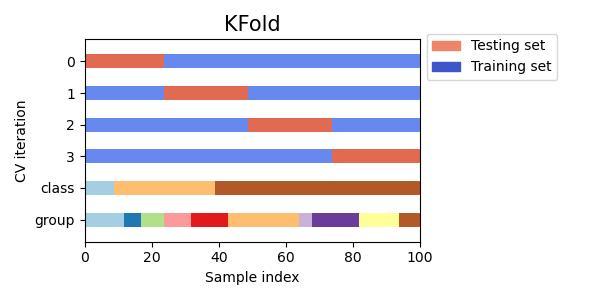
\includegraphics[width=1.0\textwidth]{../src/resources/kfold.png}
                        \caption{
                          KFold Visualization from the scikit-learn documentation \cite{scikit-learn}.
                        }
                        \label{fig:kfold}
                    \end{figure}

                    \item \textbf{Group-k-fold}: Variation of k-fold designed for situations where the data has inherent groupings or dependecies that should be preserved in the train/test split. In this method, the data is divided into \textit{K} folds, then an additional constraint is imposed to ensure that data point from the same group are in the same fold. Fig \ref{fig:groupkfold} shows the GroupKFold split.
                    
                    \begin{figure}[H]
                        \centering
                        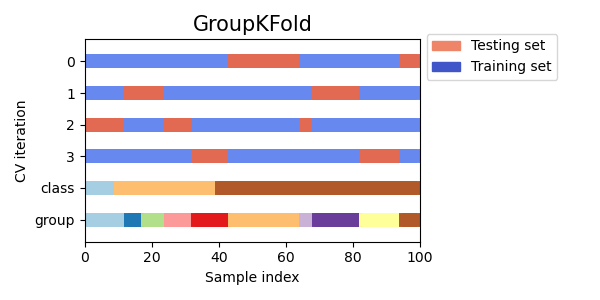
\includegraphics[width=1.0\textwidth]{../src/resources/groupkfold.png}
                        \caption{
                          GroupKFold Visualization from the scikit-learn documentation \cite{scikit-learn}.
                        }
                        \label{fig:groupkfold}
                    \end{figure}
                \end{itemize}
                
        The advantage of using \textit{Cross-Validation} over \textit{Hold-Out} is that all the samples are used for both training and testing, and each sample is used for testing exactly once. This method helps to reduce the variance of the estimated performance of the model, by averaging the results over a number of trials. The disadvantage of using Cross-Validation is that it is computationally expensive for very large datasets. \\ 

        In this study, both methods are used to evaluate the performance of the models. The Hold-Out method is used to evaluate the perfomance of the models for the \textit{Wrong approach} and \textit{Sequence approach} datasets due to their large dimension. The Cross-Validation method is used  with the Hold-Out method to evaluate the perfomance of the models for the \textit{Correct approach} and \textit{Feature Engineering approach} dataset due to them scoring the best results and being the effective approaches. Confronting the results of the two methods will show the correctness of the evaluation, as the results should be similar. \\
        
        \subsection{Metrics}

            This section will report the metrics used to benchmark the different models used in this study.

            \subsubsection{Accuracy score}

                The \textit{accuracy} is the proportion of correct predictions, considering both true positives and true negatives, among the total number of samples. The formula used to calculate the accuracy is the following:
                \begin{equation}
                    \frac{TP + TN}{TP + TN + FP + FN}
                \end{equation} 
                where \textbf{TP} is the number of true positives, \textbf{TN} is the number of true negatives, \textbf{FP} is the number of false positives and \textbf{FN} is the number of false negatives.

            \subsubsection{Precision score}

                The \textit{precision} is the ability of the classifier not to label as positive a sample that is negative. The formula used to calculate the precision is the following:
                \begin{equation}
                    \frac{TP}{TP + FP}
                \end{equation}

            \subsubsection{Recall score}

                The \textit{recall} is the ability of the classifier to find all the positive samples. The formula used to calculate the recall is the following:
                \begin{equation}
                    \frac{TP}{TP + FN}
                \end{equation}

            \subsubsection{F1 score}

                The \textit{F1 score} is the harmonic mean of the precision and recall. The formula used to calculate the F1 score is the following:
                \begin{equation}
                    \frac{ 2 \times (precision \times recall)}{precision + recall}
                \end{equation}

            \subsubsection{Matthews correlation coefficent} 

                The \textit{Matthews correlation coefficent} (or $\varphi$ coefficient) takes into account true and false positives and negatives and is regarded as a balanced measure which can be used even if the classes are of very different sizes. The formula used to calculate the $\varphi$ coefficient is as follows: 
                \begin{equation}
                    \frac{TP \times TN - FP \times FN}{\sqrt{(TP + FP)(TP + FN)(TN + FP)(TN + FN)}}
                \end{equation}

            These metrics will be used to show the effectiveness of the approaches proposed in this thesis.
    
\section{Results}
        
        Combining the validation methods and metrics presented above, the following tables will show the results obtained from the expirements conducted. The results are divided into two categories: \textbf{Exploratory} shows two approaches that were tested but did not obtain good results due to wrong implementation or loss of information. \textbf{Effective} shows two approaches that obtained good results and are suitable for this task. The results are presented in the following order: \textit{Traditional approach}, \textit{Sequence approach}, \textit{Effective approach} and \textit{Feature Engineering approach}. 

        \subsection{Exploratory}

            The following approaches are included because they are a starting point in this thesis, and show how different implementations can affect the accuracy of the models.
            
            \subsubsection{Traditional approach}
                
                Pesented in Section \ref{sec:badsplit}, it was the first one to be tested and it got surprisingly good results. Such a simple approach and yet high accuracy raised doubts about the validity of the results, after further investigation it was discovered that the dataset was not properly split into training and testing sets. 
            
                \begin{table}[htbp]
                    \centering
                    \caption{Evaluation results using \textbf{Hold-Out} validation method.}
                    \label{tab:wrong_approach_holdout}
                    \begin{tabular}{lrrrrr}
                        \toprule
                        \textbf{Model} & \textbf{Accuracy} & \textbf{F1} & \textbf{Recall} & \textbf{Precision} & \textbf{MCC} \\
                        \midrule
                        Random Forest & \textbf{0.99} & \textbf{0.99} & \textbf{0.99} & \textbf{0.99} & \textbf{0.99} \\
                        K-Nearest Neighbors & 0.98 & 0.98 & 0.98 & 0.98 & 0.98 \\
                        Decision Trees & 0.96 & 0.96 & 0.96 & 0.96 & 0.96 \\
                        Support-Vector Machines & 0.87 & 0.86 & 0.85 & 0.86 & 0.86 \\
                        Logistic Regression & 0.82 & 0.80 & 0.80 & 0.80 & 0.80 \\
                        \bottomrule
                    \end{tabular}
                \end{table}

                In Table \ref{tab:wrong_approach_holdout} the results obtained from the Hold-Out method are displayed. High values are obtained for all the metrics, with \textbf{Random Forest} obtaining the highest values with a score of \textbf{0.99} for accuracy. This confirmed the doubts about the validity of the results, a patient is both present in the training and testing set. This led to the models overfitting the data and obtaining high accuracy.

            \subsubsection{Sequence approach}

                Presented in Section \ref{sec:seqsplit}, it achieved the lowest results of all the approaches. Tested to see if by concatenating the frames of a movement into a sequence would help the models differentiate between movements and obtain a higher accuracy. 
                
                \begin{table}[htbp]
                    \centering
                    \caption{Evaluation results using \textbf{Hold-Out} validation method.}
                    \label{tab:sequence_approach_holdout}
                    \begin{tabular}{lrrrrr}
                        \toprule
                        \textbf{Model} & \textbf{Accuracy} & \textbf{F1} & \textbf{Recall} & \textbf{Precision} & \textbf{MCC} \\
                        \midrule
                        K-Nearest Neighbors & \textbf{0.56} & \textbf{0.54} & \textbf{0.54} & \textbf{0.54} & \textbf{0.51} \\
                        Random Forest & 0.55 & 0.52 & 0.53 & 0.53 & 0.49 \\
                        Support-Vector Machines& 0.52 & 0.47 & 0.49 & 0.46 & 0.47 \\
                        Logistic Regression & 0.44 & 0.41 & 0.42 & 0.43 & 0.38 \\
                        Decision Trees & 0.41 & 0.38 & 0.39 & 0.40 & 0.34 \\
                        \bottomrule
                    \end{tabular}
                \end{table}

                In Table \ref{tab:sequence_approach_holdout} the results obtained from the Hold-Out method are displayed. Low values are obtained for all the metrics, with \textbf{K-Nearest Neighbor} obtaining the highest values with a score of \textbf{0.56} for accuracy. This results are considered low based on other approaches, however in the context of randomly guessing the movement of a patient the accuracy would be \textbf{0.10} as there are 10 movements. This means that the models are able to differentiate between movements, but the sequence implementation leads to a loss of information and a high accuracy cannot be obtained.

        \subsection{Effective}

                The following approaches are the ones that obtained the best results and are suitable for this task. The main difference between the two approaches is the data used to train the models. The \textit{Correct Approach} uses the data as it is from the Kinect sensor, while the \textit{Feature Engineering Approach} uses the data after applying feature engineering techniques.
                
            \subsubsection{Correct approach}

                Presented in Section \ref{sec:goodsplit}, considered effective because the raw kinect data is able to obtain a high accuracy. The data is not modified in any way, beside the removal of rotational , state  and pre-processing the data to remove noise and outliers.\\
                 
                In Table \ref{tab:correct_approach_holdout} the results obtain from the Hold-Out method are shown. \textbf{Random Forest} obtains the highest values for all the metrics, with a score of \textbf{0.74} for accuracy. Other models such as \textit{Gradient Boosting}, \textit{Linear Discriminant Analysis}, \textit{Support-Vector Machines}, \textit{K-Nearest Neighbors} obtained great results as well with a score greater than \textbf{0.70} for accuracy. This confirms that the data obtained from the Kinect sensor is suitable for the task of movement classification without any major tweaks.\\
                
                \newpage

                \begin{table}[htbp]
                    \centering
                    \caption{Evaluation results using \textbf{Hold-Out} validation method.}
                    \label{tab:correct_approach_holdout}
                    \begin{tabular}{lrrrrr}
                        \toprule
                        \textbf{Model} & \textbf{Accuracy} & \textbf{F1} & \textbf{Recall} & \textbf{Precision} & \textbf{MCC} \\
                        \midrule
                        Random Forest & \textbf{0.74} & \textbf{0.73} & \textbf{0.73} & \textbf{0.73} & \textbf{0.71} \\
                        Gradient Boosting & 0.73 & 0.72 & 0.72 & 0.72 & 0.69 \\
                        Linear-Discriminant Analysis & 0.72 & 0.71 & 0.71 & 0.74 & 0.68 \\
                        Support-Vector Machines & 0.71 & 0.71 & 0.71 & 0.72 & 0.68 \\
                        K-Nearest Neighbors & 0.71 & 0.69 & 0.69 & 0.70 & 0.67 \\
                        Logistic Regression & 0.66 & 0.64 & 0.64 & 0.64 & 0.62 \\
                        Multi-Layer Perceptron & 0.63 & 0.59 & 0.62 & 0.61 & 0.59 \\
                        Naive Bayes & 0.63 & 0.60 & 0.61 & 0.62 & 0.58 \\
                        Decision Trees & 0.63 & 0.60 & 0.62 & 0.61 & 0.58 \\
                        Ada Boost & 0.35 & 0.22 & 0.28 & 0.24 & 0.32 \\
                        \bottomrule
                    \end{tabular}
                \end{table}

                In Table \ref{tab:correct_approach_holdout} \textbf{Hold-Out} validation method was used for all the models, while in Table \ref{tab:correct_approach_cv} \textbf{Cross-Validation} was used with only 3 models to compare the two validation methods and show that there is no major difference between them. The results obtained from the two methods are similar. \\

                Hold-Out method was used for it's speed, with \textbf{10 minutes} of training time while cross-validation run for hours without finishing. This is due to the fact that this approaches use the raw Kinect data, that contains over \textbf{59000} rows and \textbf{100} columns. 
                
                \begin{table}[htbp]
                    \centering
                    \caption{Comparison of obtained results with Cross-Validation and Hold-Out methods. The metrics reported are (from top to bottom): Accuracy, F1, Recall, Precision, MCC.}
                    \label{tab:correct_approach_cv}
                    \begin{tabular}{|c|c|c|}
                    \hline
                    \textbf{Model} & \textbf{Cross-Validation} & \textbf{Hold-Out} \\ \hline
                        Linear Discriminant Analysis    & 0.73 & 0.72 \\ 
                                                        & 0.71 & 0.71 \\ 
                                                        & 0.70 & 0.71 \\ 
                                                        & 0.75 & 0.74 \\
                                                        & 0.70 & 0.68 \\ 
                                                        \hline
                        K-Nearest Neighbors             & 0.71 & 0.71 \\ 
                                                        & 0.70 & 0.69 \\ 
                                                        & 0.70 & 0.69 \\ 
                                                        & 0.71 & 0.70 \\
                                                        & 0.68 & 0.67 \\
                                                        \hline
                        Naive Bayes                     & 0.66 & 0.63 \\ 
                                                        & 0.62 & 0.60 \\ 
                                                        & 0.63 & 0.62 \\
                                                        & 0.66 & 0.61 \\ 
                                                        & 0.62 & 0.58 \\ 
                                                        \hline
                    \end{tabular}
                \end{table}
                
                In Table \ref{tab:correct_approach_mat_hoop} are displayed the results of a final approach, where two movements \textit{Mat-Walk} and \textit{Hoop-Walk} are removed from the dataset one at a time. The results show that the accuracy of the models increased by \textbf{4\%} to \textbf{5\%}. This is due to the fact that the two movements are very similar, and this caused the models to struggle to differentiate between them no matter the features used. \\
                By removing either one of the movements, the models accuracy increased by the same amount. This leaves the decision to the user to choose which movement to remove based on the context of the application. 

                \begin{table}[htbp]
                    \centering
                    \caption{Comparison of obtained results with Mat-Walk and Hoop-Walk removed from the dataset. The metrics reported are (from top to bottom): Accuracy, F1, Recall, Precision, MCC.}
                    \label{tab:correct_approach_mat_hoop}
                    \begin{tabular}{|c|c|c|}
                    \hline
                    \textbf{Model} & \textbf{Hoop Walk Removed} & \textbf{Mat Walk Removed} \\ \hline
                        Random Forest                   & 0.79 & 0.79 \\ 
                                                        & 0.79 & 0.79 \\ 
                                                        & 0.79 & 0.79 \\ 
                                                        & 0.79 & 0.79 \\
                                                        & 0.76 & 0.76 \\ 
                                                        \hline
                        Gradient Boosting               & 0.78 & 0.78 \\ 
                                                        & 0.78 & 0.78 \\ 
                                                        & 0.78 & 0.78 \\ 
                                                        & 0.78 & 0.79 \\
                                                        & 0.74 & 0.75 \\
                                                        \hline
                        Linear-Discriminant Analysis    & 0.76 & 0.76 \\ 
                                                        & 0.77 & 0.77 \\ 
                                                        & 0.76 & 0.76 \\
                                                        & 0.80 & 0.79 \\ 
                                                        & 0.73 & 0.73 \\ 
                                                        \hline
                    \end{tabular}
                \end{table} 

           \newpage 

            \subsubsection{Feature engineering approach}
                
                Presented in Section \ref{sec:feature_engineering}, considered the most effective because it obtained the highest accuracy of all the approaches and it is the fastest to train. The data is modified by applying feature engineering techniques, this leads to the dataset having less rows and columns.
            
            \begin{table}[htbp]
                \centering
                \caption{Evaluation results using \textbf{Cross-Validation} method.}
                \label{tab:feature_engineering_approach_cv}
                \begin{tabular}{lrrrrr}
                    \toprule
                    \textbf{Model} & \textbf{Accuracy} & \textbf{F1} & \textbf{Recall} & \textbf{Precision} & \textbf{MCC} \\
                    \midrule
                    Multi-Layer Perceptron & \textbf{0.83} & \textbf{0.83} & \textbf{0.84} & \textbf{0.84} & \textbf{0.81} \\
                    Logistic Regression & 0.82 & 0.83 & 0.83 & 0.84 & 0.80 \\
                    Linear-Discriminant Analysis & 0.81 & 0.82 & 0.83 & 0.84 & 0.80 \\
                    Support-Vector Machines & 0.81 & 0.82 & 0.83 & 0.83 & 0.80 \\
                    Random Forest & 0.79 & 0.80 & 0.80 & 0.82 & 0.77 \\
                    Gradient Boosting & 0.78 & 0.79 & 0.79 & 0.82 & 0.76 \\
                    K-Nearest Neighbors & 0.78 & 0.79 & 0.80 & 0.80 & 0.76 \\
                    Decision Trees & 0.73 & 0.73 & 0.74 & 0.77 & 0.70 \\
                    Naive Bayes & 0.63 & 0.63 & 0.66 & 0.66 & 0.60 \\
                    Ada Boost & 0.46 & 0.38 & 0.46 & 0.42 & 0.43 \\
                    \bottomrule
                \end{tabular}
            \end{table}

            In Table \ref{tab:feature_engineering_approach_cv} the results obtained from the Cross-Validation method are displayed. High values are obtained for all the metrics, with \textbf{Multi-Layer Perceptron}  and \textbf{Logistic Regression} obtaining the highest values with a score of \textbf{0.83} and \textbf{0.82} for accuracy. Other models such as \textit{Linear-Discriminant Analysis}, \textit{Gradient Boosting}, \textit{Random Forest}, \textit{Support-Vector Machines}, \textit{K-Nearest Neighbors} obtained great results as well with a score greater than \textbf{0.70} for accuracy. 

            \begin{table}[htbp]
                \centering
                \caption{Comparison of obtained results with Cross-Validation and Hold-Out methods. The metrics reported are (from top to bottom): Accuracy, F1, Recall, Precision, MCC.}
                \label{tab:feature_engineering_approach_holdout}
                \begin{tabular}{|c|c|c|}
                \hline
                \textbf{Model} & \textbf{Cross-Validation} & \textbf{Hold-Out} \\ \hline
                    Linear Discriminant Analysis    & 0.81 & 0.82 \\ 
                                                    & 0.82 & 0.82 \\ 
                                                    & 0.83 & 0.83 \\ 
                                                    & 0.84 & 0.83 \\
                                                    & 0.80 & 0.80 \\ 
                                                    \hline
                    Logistic Regression             & 0.82 & 0.80 \\ 
                                                    & 0.83 & 0.81 \\ 
                                                    & 0.83 & 0.82 \\ 
                                                    & 0.84 & 0.82 \\
                                                    & 0.80 & 0.78 \\
                                                    \hline
                    Multi-Layer Perceptron          & 0.83 & 0.70 \\ 
                                                    & 0.83 & 0.71 \\ 
                                                    & 0.84 & 0.71 \\
                                                    & 0.84 & 0.78 \\ 
                                                    & 0.81 & 0.68 \\ 
                                                    \hline
                \end{tabular}
            \end{table}

            \newpage

            This confirms that the feature engineering techniques applied to the data are suitable for the task of movement classification. This approach is  also the fastest to train, with a training time of \textbf{1 minute}. \\

            Table \ref{tab:feature_engineering_approach_holdout} shows the results obtained from the Hold-Out validation method. Similar to the ones obtained with Cross-Validation method, with a lower training time of \textbf{10 seconds}. However, Cross-Validation is preferred over Hold-Out because it is more used in the literature and robust.\\

            In Table \ref{tab:feature_engineering_approach_mat_hoop} are displayed the results of the final approach used in the Correct approach. The results show that the accuracy of the models increased by \textbf{8\%} to \textbf{12\%}. This is a larger increse than the one obtained in the Correct approach, this is due to the fact that the feature engineering techniques applied are more informative than the raw Kinect data. Leading to the models being able to differentiate between the two movements more easily. \\

            \begin{table}[htbp]
                \centering
                \caption{Comparison of obtained results with Mat-Walk and Hoop-Walk removed from the dataset. The metrics reported are (from top to bottom): Accuracy, F1, Recall, Precision, MCC.}
                \label{tab:feature_engineering_approach_mat_hoop}
                \begin{tabular}{|c|c|c|}
                \hline
                \textbf{Model} & \textbf{Hoop Walk Removed} & \textbf{Mat Walk Removed} \\ \hline
                    Multi-Layer Perceptron          & 0.90 & 0.91 \\ 
                                                    & 0.90 & 0.91 \\ 
                                                    & 0.90 & 0.92 \\
                                                    & 0.92 & 0.92 \\ 
                                                    & 0.89 & 0.90 \\
                                                    \hline
                    Logistic Regression             & 0.90 & 0.91 \\ 
                                                    & 0.91 & 0.91 \\ 
                                                    & 0.91 & 0.91 \\ 
                                                    & 0.92 & 0.92 \\
                                                    & 0.89 & 0.90 \\
                                                    \hline
                    Linear Discriminant Analysis    & 0.91 & 0.90 \\ 
                                                    & 0.91 & 0.91 \\ 
                                                    & 0.91 & 0.91 \\ 
                                                    & 0.92 & 0.92 \\
                                                    & 0.90 & 0.89 \\ 
                                                    \hline
                \end{tabular}
            \end{table}

\newpage
            
\section{Discussion}
        
        This section will discuss the results obtained from the expirements conducted in the previous chapter. The difference between the approaches, the best performing models and the similarity between movements will be the topic of discussion. 

        \subsubsection{Differences between approaches}
            Four approaches were tested in this thesis, each one with a diffrent implementation. It was presented that \textit{Feature engineering} obtained the best results in terms of accuracy and training time. However, the \textit{Correct approach} also obtained great results but it was laking in training time. These two approaches were considere the most effective and suitable for the task of movement classification. Nevertheless, their implementation is completely different, with one using the raw Kinect data containing a very large number of rows and columns, while the other uses the data after applying feature engineering techniques transforming the data into a more informative dataset. This demonstrates how the approach used to solve a problem can affect the results obtained. 
            The others two approaches \textit{Wrong approach} and \textit{Sequence approach}
            prove that an incorrect data splitting method and a loss of information can lead to low accuracy. Their implementation is not suitable for this task but were a crucial step in the development phase to better understand why the models were not performing well. 

        \subsubsection{Best performing models}
            The models listed below obtained the best results in the two approaches considered effective. 

            \begin{boxlabel}
                \item \textbf{Random Forest} and \textbf{Gradient Boosting} are the two best performing models in the \textit{Correct approach} with a \textbf{0.74} and \textbf{0.73} accuracy score respectively.
                \item \textbf{Multi-Layer Perceptron} and \textbf{Logistic Regression} are the two best performing models in the \textit{Feature engineering approach} with a \textbf{0.83} and \textbf{0.82} accuracy score.
            \end{boxlabel}

            The results above demonstrate how the models perform differently depending on the approach used, due to the fact that the used to train the models is of different dimension and information. 

        \subsubsection{Movements similarity}   
        
            It was demonstrated in Table \ref{tab:correct_approach_mat_hoop} and Table \ref{tab:feature_engineering_approach_mat_hoop} that by removing \textit{Mat-Walk} and \textit{Hoop-Walk} from the dataset, the accuracy of the models increased.

            This problem was first noticed when the confusion matrix was plotted for the \textit{Feature enginerring} approach using the \textit{Multi-Layer Perceptron} model. In
            Figure \ref{fig:cm_all} the Confusion Matrix of all 10 movements is displayed, the model is struggling to differentiate between movement 3 and 5 (Mat-Walk and Hoop-Walk). In Figure \ref{fig:cm_remove} one between Mat-Walk and Hoop-Walk is removed, the model does not struggle anymore to differentiate between the two movements.
            
            \begin{figure}[h]
                \begin{subfigure}{.5\textwidth}
                \centering
                  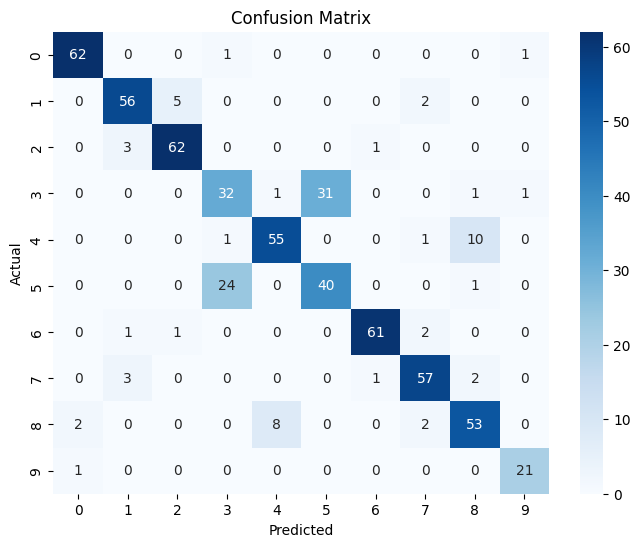
\includegraphics[width=1.\linewidth]{../src/resources/plots/fe.png}
                  \caption{10 Movements.}
                  \label{fig:cm_all}
                \end{subfigure}%
                \begin{subfigure}{.5\textwidth}
                \centering
                  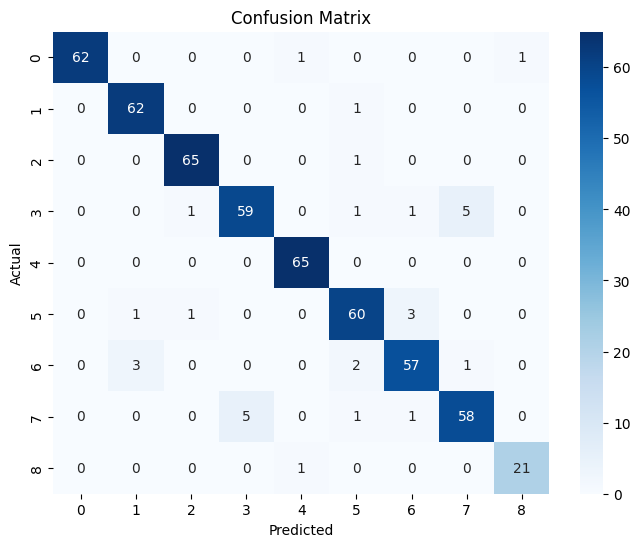
\includegraphics[width=1.\linewidth]{../src/resources/plots/fe-remove.png}
                  \caption{9 Movements.}
                  \label{fig:cm_remove}
                \end{subfigure}
                \caption{Confusion Matrix of Multi-Layer Perceptron model using Feature Engineering approach.}
            \end{figure}
            
            \newpage

            To confirm this, \textit{3D Visualization} of the movements used in Section \ref{sec:movements_visualization} was used. A random sample of \textit{Mat-Walk} and \textit{Hoop-Walk} was plotted, in Figure \ref{fig: hoop-walk} and Figure \ref{fig: mat-walk} the two movements are displayed. The two movements are very similar due to the fact that they are both walking movements, the only difference is that in \textit{Mat-Walk} the patient is walking on a mat while in \textit{Hoop-Walk} the patient is walking in a hoop. This is the reason why the models struggle to differentiate between the two movements.

            \begin{figure}[h]
                \begin{subfigure}{.5\textwidth}
                \centering
                  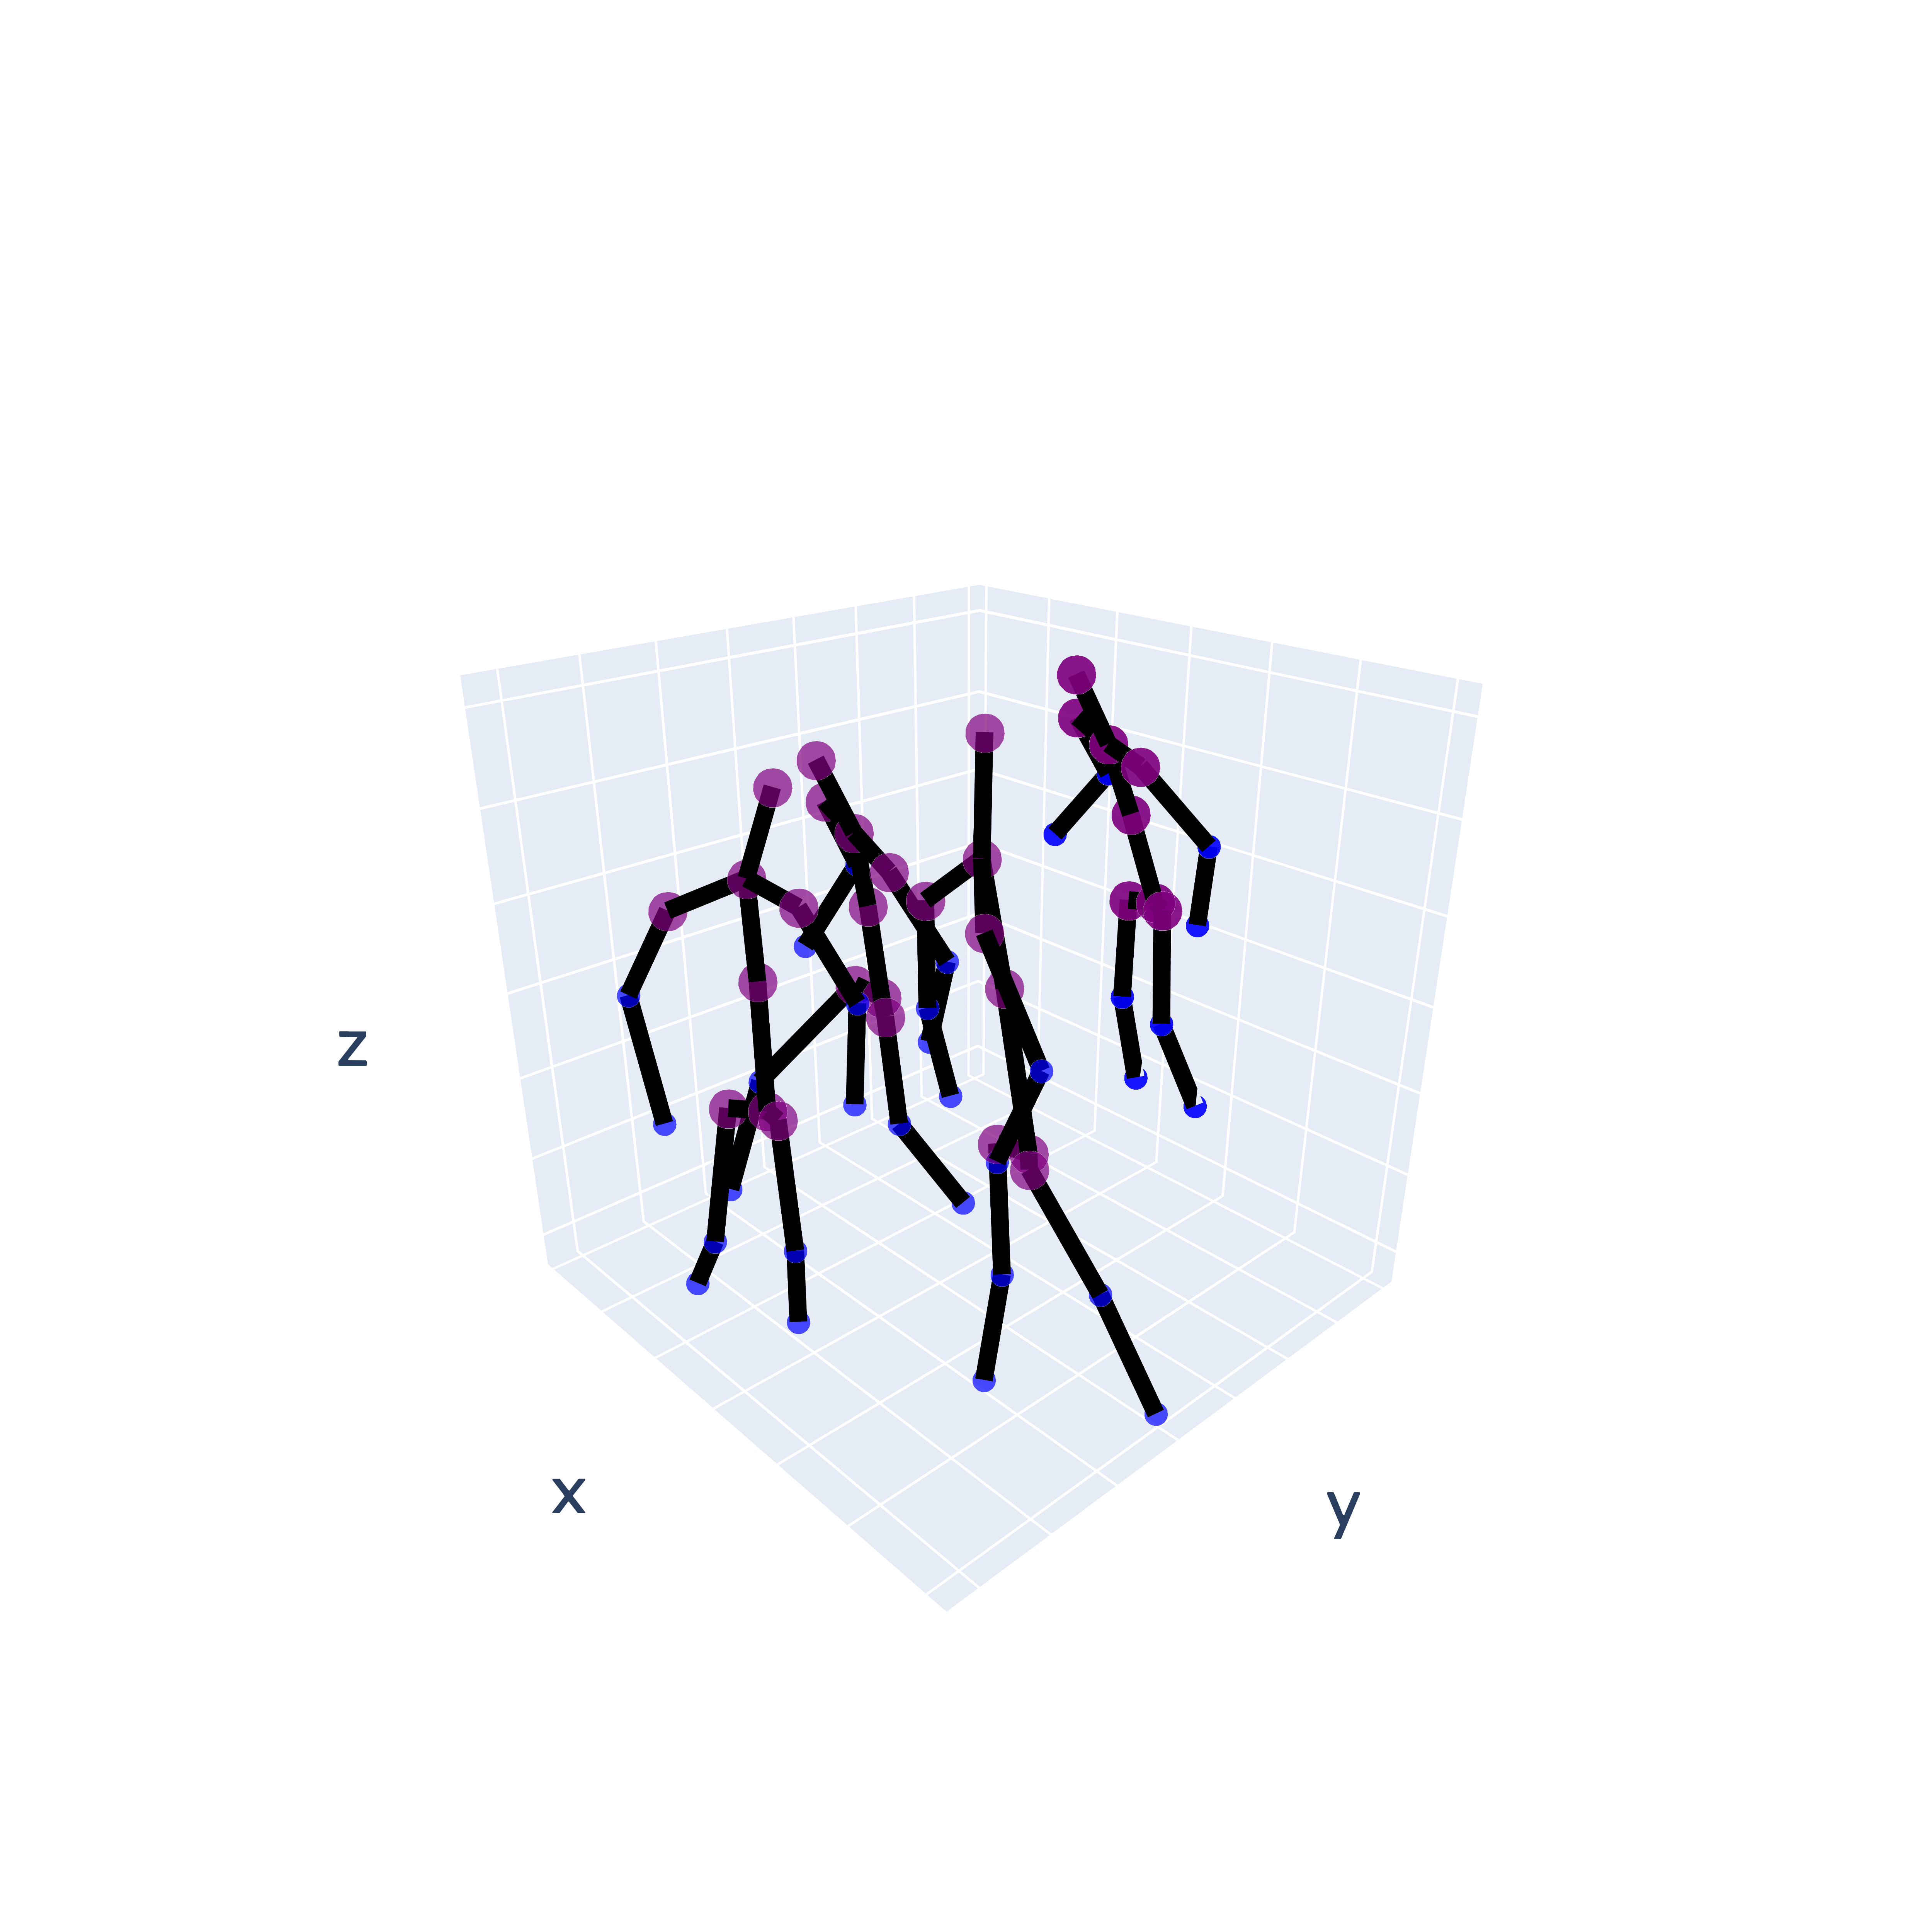
\includegraphics[width=1.\linewidth]{../src/resources/mov-plots/mov-1.png}
                  \caption{Hoop-Walk Movement.}
                  \label{fig: hoop-walk}
                \end{subfigure}
                \begin{subfigure}{.5\textwidth}
                \centering
                  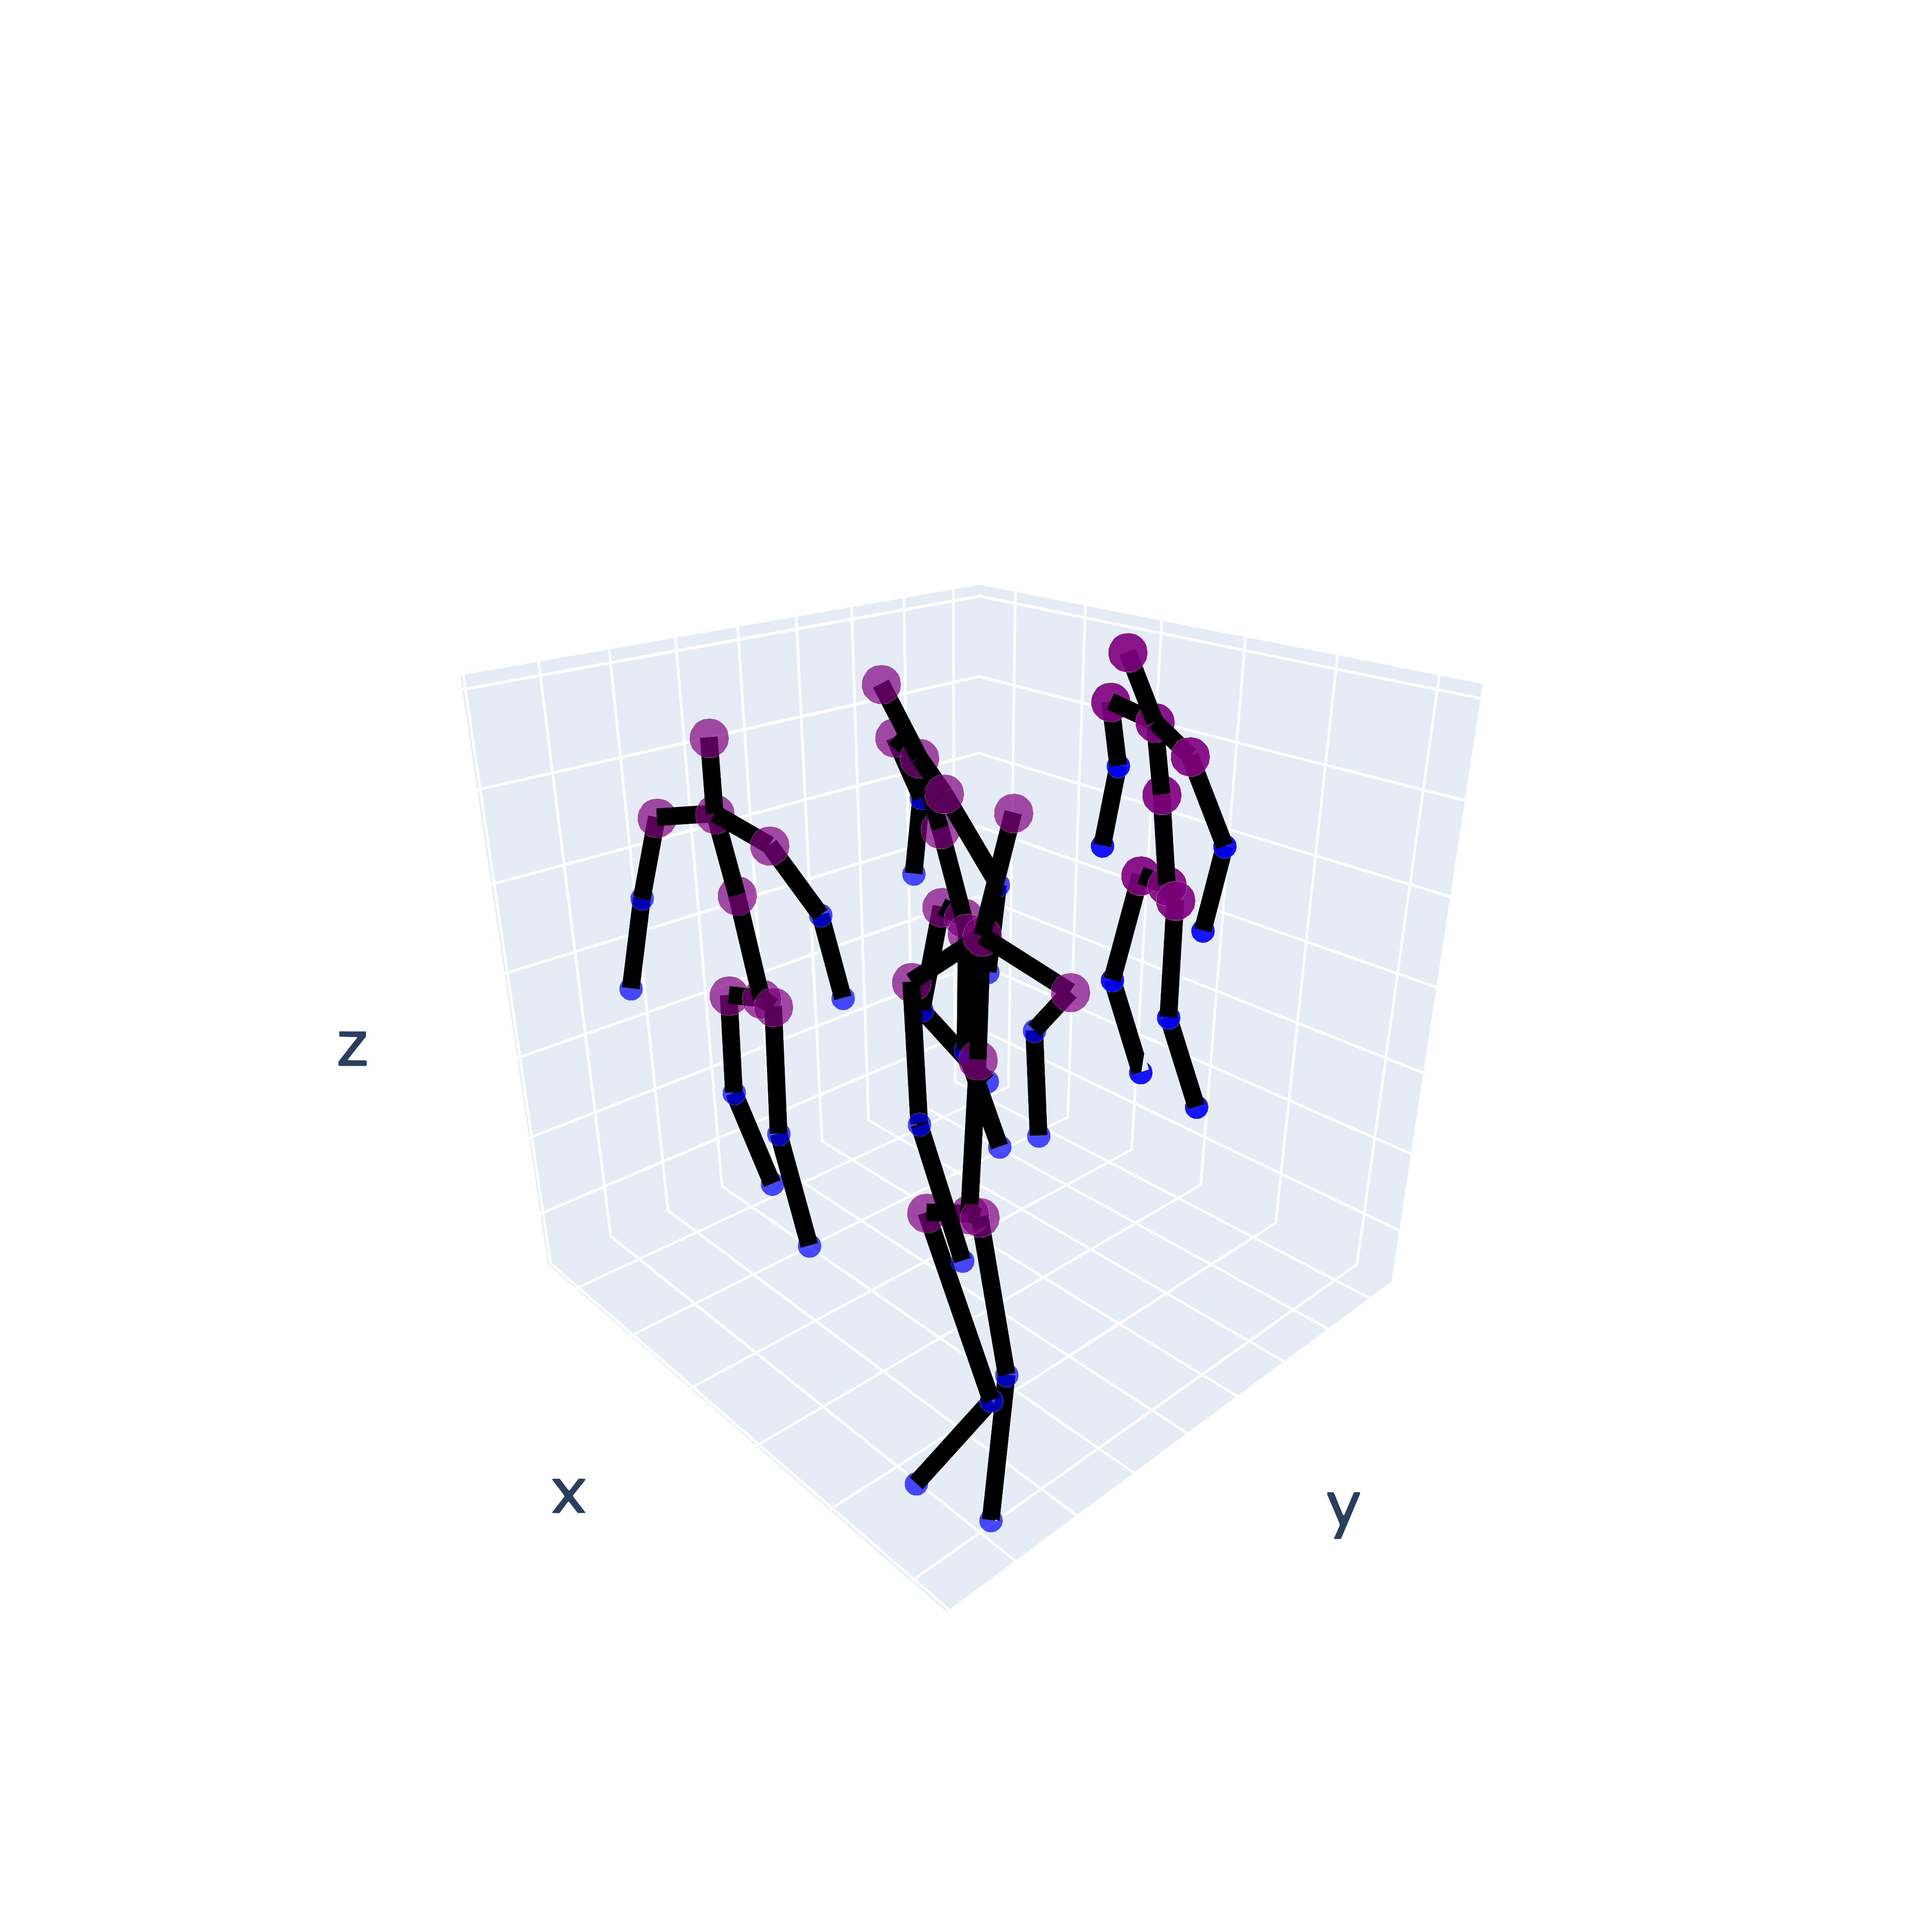
\includegraphics[width=1.\linewidth]{../src/resources/mov-plots/mov-8.png}
                  \caption{Mat-Walk Movement.}
                  \label{fig: mat-walk}
                \end{subfigure}
                \caption{3D Visualization plots of the two similar movements.}
            \end{figure}

\cleardoublepage